\documentclass[t, 10pt, aspectratio=169, table, x11names]{beamer}
\usetheme{metropolis}

\usepackage{xcolor}
\usepackage[utf8]{inputenc}
\usepackage[default]{lato}
\usepackage[T1]{fontenc}
\usepackage{lmodern}
\usepackage{listingsutf8}
\usepackage{hyperref}
\usepackage{wrapfig}
\usepackage{dsfont}
\usepackage[export]{adjustbox}
\usepackage{array, booktabs}
\usepackage{cellspace}

\graphicspath{{./resources}}
\lstset{inputpath=./resources, xleftmargin=7mm, xrightmargin=7mm}

\definecolor{codegreen}{rgb}{0,0.6,0}
\definecolor{codegray}{rgb}{0.5,0.5,0.5}
\definecolor{codepurple}{rgb}{0.58,0,0.82}
\definecolor{backcolour}{rgb}{0.95,0.95,0.92}
\hypersetup{colorlinks,urlcolor=blue}

\newcommand{\redhighlight}[1]{{\color{red}\textbf{\texttt{#1}}}}

\newcommand{\R}{\mathds{R}}
\newcommand{\appallingunderline}[1]{
	\underline{\smash{#1}\vphantom{T}}\vphantom{#1}%
}

\lstdefinestyle{sql}{
	backgroundcolor=\color{backcolour},
	commentstyle=\color{codegreen},
	keywordstyle=\color{magenta},
	numberstyle=\tiny\color{codegray},
	stringstyle=\color{codepurple},
	basicstyle=\ttfamily\scriptsize,
	breakatwhitespace=false,
	breaklines=true,
	captionpos=b,
	keepspaces=true,
	numbers=left,
	numbersep=5pt,
	showspaces=false,
	showstringspaces=false,
	showtabs=false,
	tabsize=2
}

\lstdefinestyle{winprompt}{
	backgroundcolor=\color{backcolour},
	commentstyle=\color{codegreen},
	keywordstyle=\color{magenta},
	numberstyle=\tiny\color{codegray},
	stringstyle=\color{codepurple},
	basicstyle=\ttfamily\footnotesize,
	breakatwhitespace=false,
	breaklines=false,
	breakatwhitespace=false,
	prebreak=false,
	captionpos=b,
	keepspaces=true,
	showspaces=false,
	showstringspaces=false,
	showtabs=false,
	tabsize=1
}

\lstset{style=sql}
\lstset{inputencoding=utf8/latin1}


\begin{document}

	\author{Victor Mayrink}
	\title{Curso de SQL}
	\subtitle{Aula 1: Instalação das ferramentas e configuração do ambiente}

	%Frame: title
	\begin{frame}[plain]
		\maketitle
	\end{frame}
	
	%Frame: agenda
	\begin{frame}
		\frametitle{Resumo da aula}
		\vspace{0.5cm}
		\begin{figure}[h]
			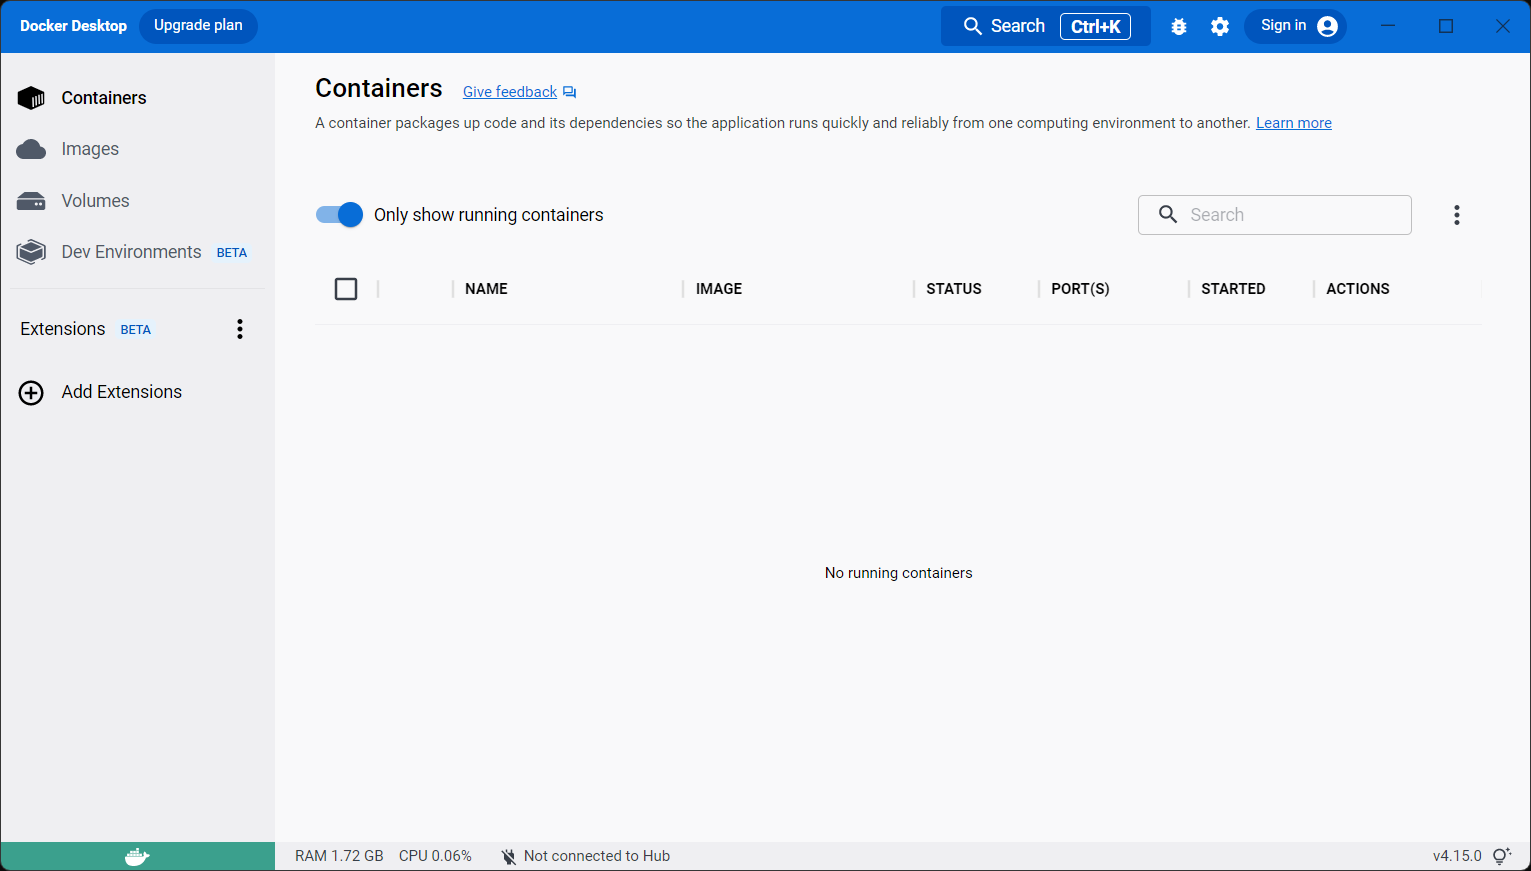
\includegraphics[width=0.70\textwidth]{docker-window.png}
		\end{figure}
	\end{frame}

	%Frame: client-server
	\begin{frame}
		\frametitle{Arquitetura cliente-servidor}
		A comunicação com o banco de dados, ocorre em um esquema \textbf{cliente-servidor}
		\vspace{3mm}
		\begin{figure}[h]
			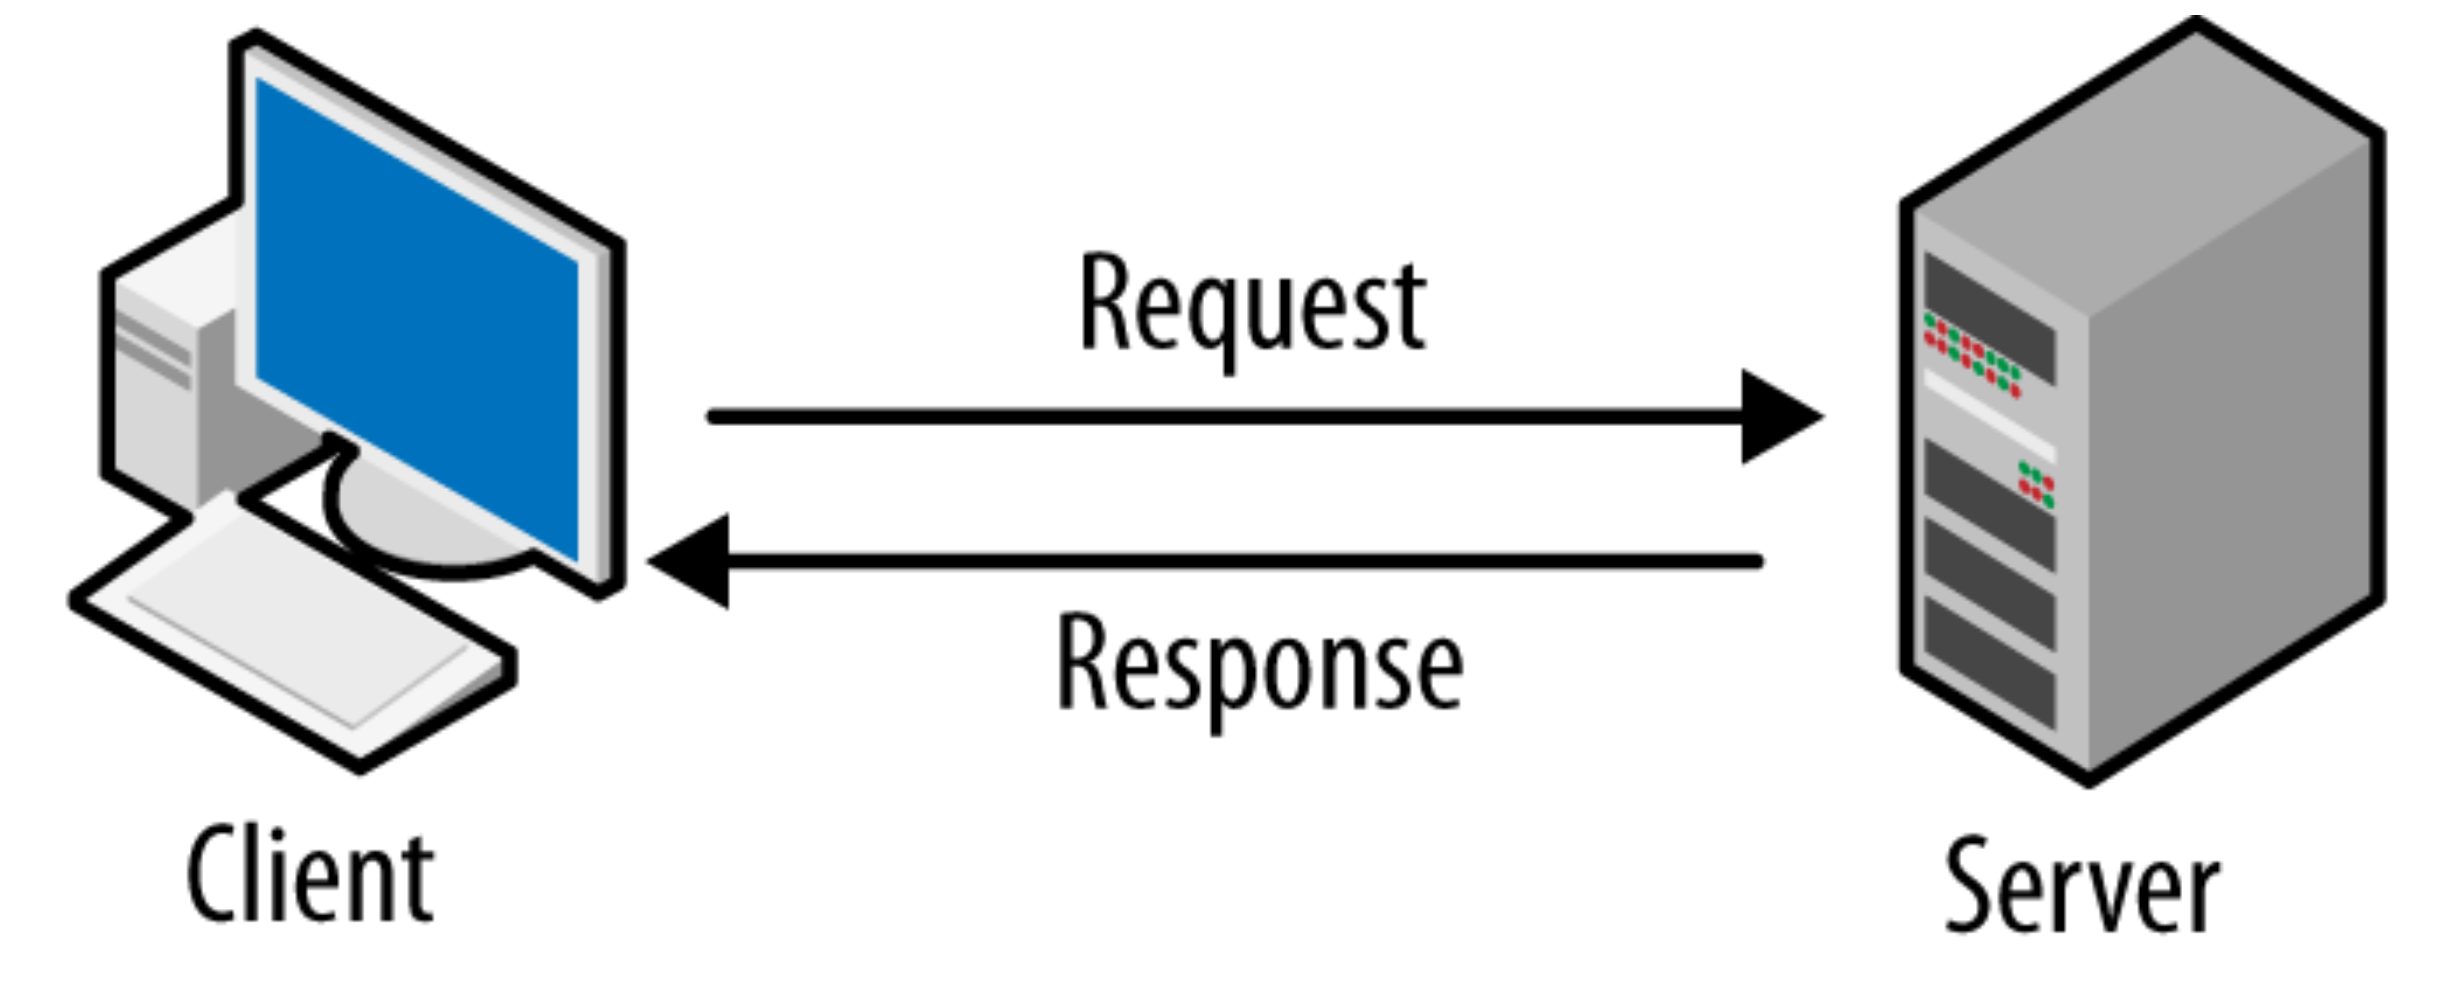
\includegraphics[width=0.60\textwidth]{client-server-diagram.png}
		\end{figure}
		\begin{itemize}
			\item O cliente envia uma \textbf{requisição} (ou comando)
			\item O servidor executa o comando e retorna uma \textbf{resposta}
		\end{itemize}
	\end{frame}
	
	%Frame: database clients
	\begin{frame}
		\frametitle{Clientes de bancos de dados}
		Existem diferentes \textit{softwares} que funcionam como clientes de bancos de dados
		\medskip
		\begin{itemize}
			\item DBeaver
			\item MySQL workbench
			\item DataGrip
			\item DbVisualizer
		\end{itemize}
		\begin{figure}
			\vspace{2mm}
			\centering
			
\includegraphics[height=15mm]{dbeaver.png}
			\hspace{10mm}
			
\includegraphics[height=15mm]{logo-mysql-workbench}
			\hspace{10mm}
			
\includegraphics[height=15mm]{logo-datagrip.png}
			\hspace{7mm}
			
\includegraphics[height=15mm]{logo-dbvis.png}
		\end{figure}
	\end{frame}

	%Frame: database servers
	\begin{frame}
		\frametitle{Servidores de bancos de dados}
		\begin{itemize}
			\item[] Da mesma forma, também existem diferentes \textit{softwares} que funcionam como servidores de banco de dados
			\bigskip\bigskip
			\begin{table}
				\begin{center}
					\begin{tabular}{cccc}
						
\includegraphics[height=14mm]{logo-postgres} &
						
\includegraphics[height=14mm]{logo-mysql} &
						
\includegraphics[height=14mm]{logo-mariadb} &
						
\includegraphics[height=14mm]{logo-redshift}
						\\ \\ \\
						
\includegraphics[height=14mm]{logo-snowflake} &
						
\includegraphics[height=14mm]{logo-sql-server} &
						
\includegraphics[height=14mm]{logo-sqllite} &
						
\includegraphics[height=14mm]{logo-hive}
					\end{tabular}
				\end{center}
			\end{table}
		\end{itemize}
	\end{frame}

	%Frame: client-server
	\begin{frame}
		\frametitle{Arquitetura cliente-servidor}
		Normalmente, o servidor e o cliente rodam em máquinas diferentes e se comunicam via internet. 
		\begin{figure}[h]
			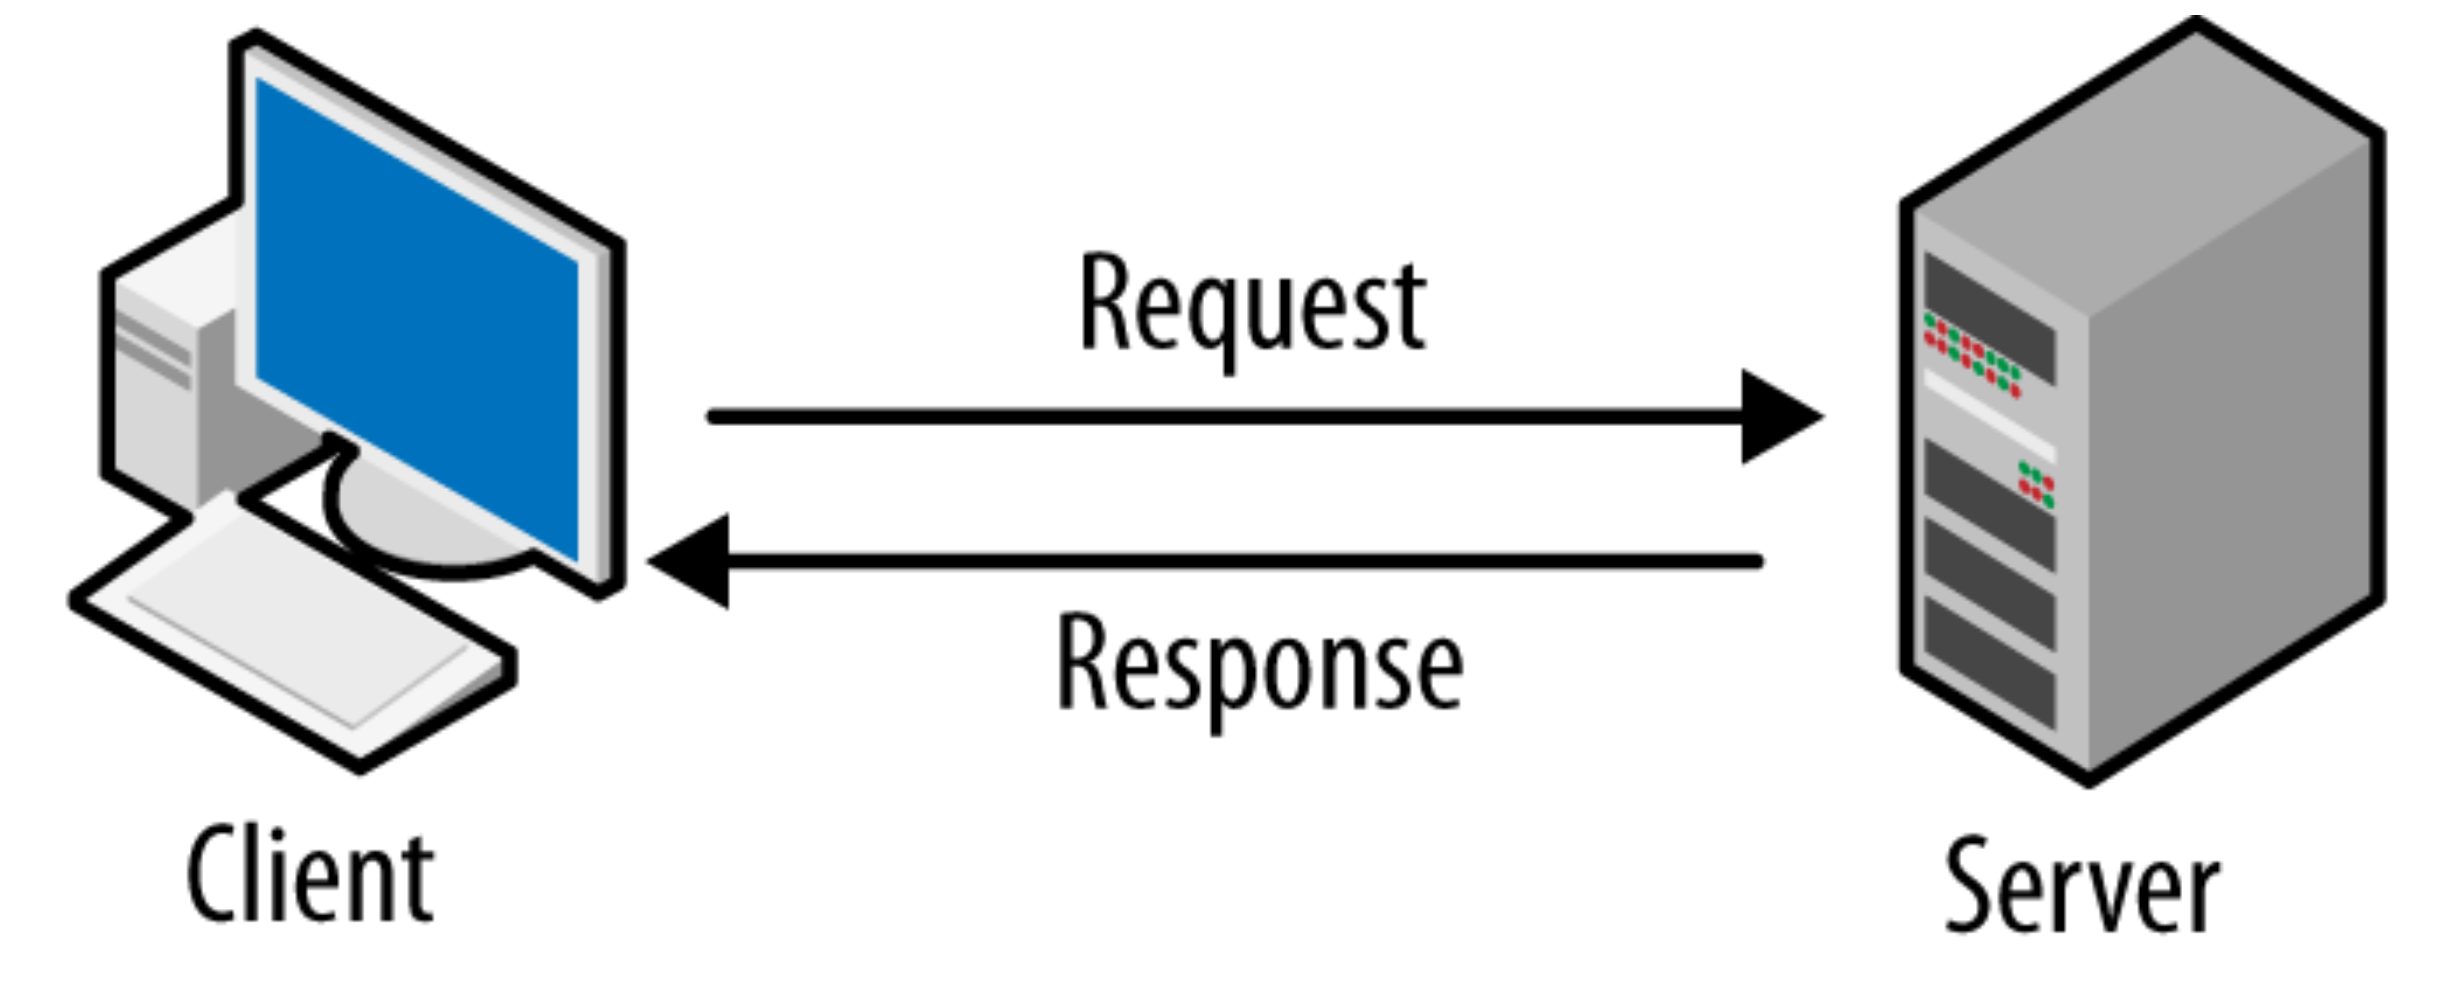
\includegraphics[width=0.50\textwidth]{client-server-diagram.png}
		\end{figure}
		\begin{itemize}
			\item[] Caso geral:
			\begin{itemize}
				\item O cliente é o nosso computador trabalho
				\item O servidor é um banco de dados rodando na nuvem (AWS, GCP, Azure, UolHost, etc...)
			\end{itemize}
			\vspace{2mm}
			\item[] No nosso caso vamos simular um servidor na nossa própria máquina de trabalho. 
		\end{itemize}
	\end{frame}

	\section{Bora começar!?}

	\begin{frame}
		\frametitle{Requisitos}
		Para fazer atividades do curso, precisamos instalar o cliente e servidor no nosso computador de trabalho.
		\begin{columns}[t]
			\begin{column}{0.20\textwidth}
				\vspace{0.3cm}
				\begin{figure}[h]
					
\includegraphics[width=1.5cm, right]{dbeaver.png}
				\end{figure}
				\vspace{1.1cm}
				\begin{figure}[h]
					
\includegraphics[width=1.5cm, right]{docker.png}
				\end{figure}
			\end{column}

			\begin{column}{0.70\textwidth}
				\begin{itemize}
					\item \textbf{Dbeaver}: \href{https://dbeaver.io/download}{ \appallingunderline{https://dbeaver.io/download}}
					\begin{itemize}
						\item Interface amigável
						\item Múltiplas funcionalidades
						\item Suporta diferentes tipos de bancos de dados
					\end{itemize}

					\vspace{0.4cm}
					\item \textbf{Docker}: \href{https://www.docker.com/products/docker-desktop/}{\appallingunderline{https://www.docker.com/products/docker-desktop/}}
					
					\begin{itemize}
						\item Utilizaremos o Docker para simular um \textit{servidor} de banco de dados no nosso próprio computador
						\item Além do Docker, vamos precisar da \textit{imagem} do banco de dados que iremos executar
					\end{itemize}
				\end{itemize}
			\end{column}
			\begin{column}{0.05\textwidth}
			\end{column}
		\end{columns}
	\end{frame}

	\section{Instalação do Dbeaver}

	%Frame: dbeaver installation #1
	\begin{frame}
		\frametitle{Instalação Dbeaver}
		A instalação do Dbeaver é relativamente simples. Baixe o instalador e siga o fluxo de instalação normalmente utilizando as configurações recomendadas e pré-definidas.
		\begin{figure}[h]
			\centering\vspace{2mm}
			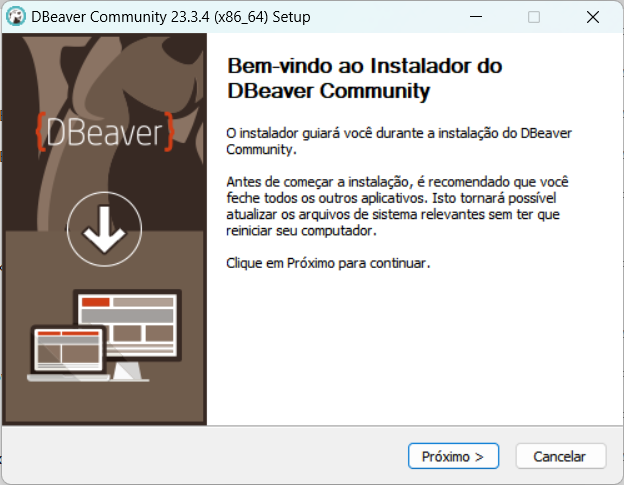
\includegraphics[width=0.45\textwidth]{dbeaver-install-start.png}
			\hspace{0.5cm}
			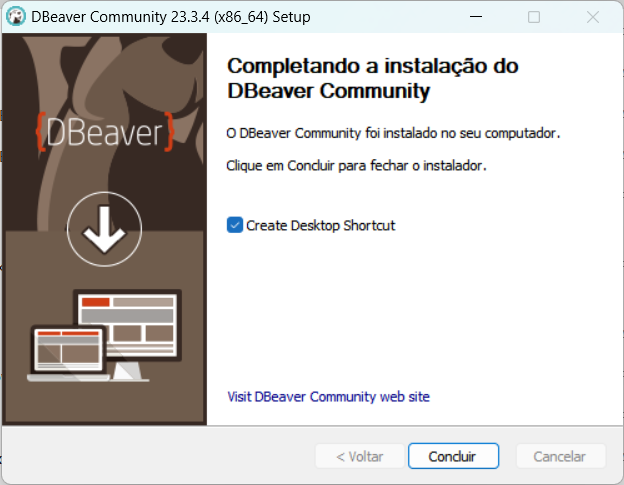
\includegraphics[width=0.45\textwidth]{dbeaver-install-finish.png}
		\end{figure}
	\end{frame}
	
	%Frame: dbeaver installation #2
	\begin{frame}
		\frametitle{Instalação Dbeaver}
		Depois de instalado. Esta é a aparência do Dbeaver:
		\begin{figure}[h]
			\centering\vspace{2mm}
			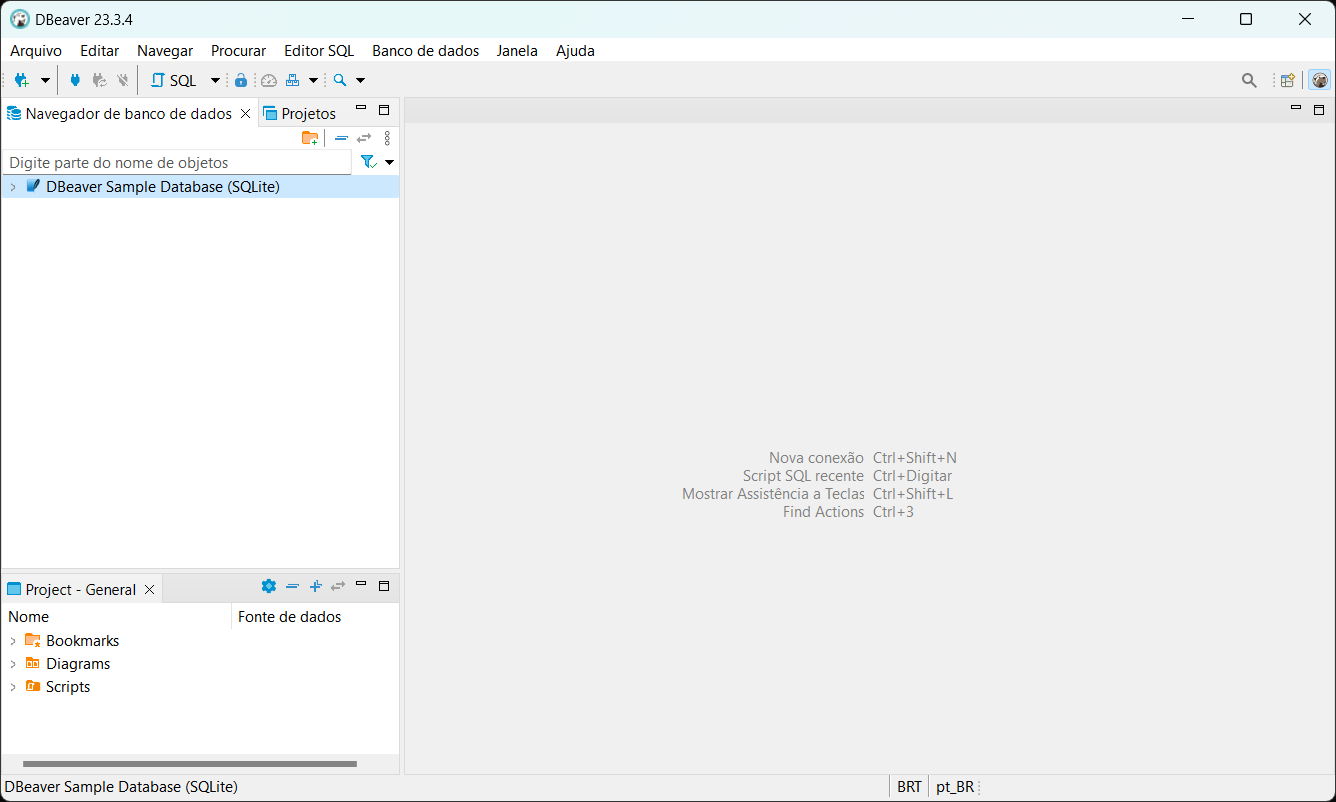
\includegraphics[width=0.70\textwidth]{dbeaver-window.png}
		\end{figure}
	\end{frame}

	\section{Instalação do Docker}

	\begin{frame}
		\frametitle{O que é Docker?}
		O que é \textit{esse tal} de Docker?
		\vspace{3mm} 
		\begin{itemize}
			\item O Docker é um software de código aberto usado para exectutar aplicações dentro de \textbf{containers} virtuais.
			\vspace{2mm}
			\item A maior parte das aplicações são projetadas e otimizadas para rodar em um SO específico e possuem dependências de bibliotecas de sistema.
			\vspace{2mm}
			\item Com o Docker, é possível emular uma aplicações projetada para rodar em outro SO e sem se preocupar com a instalação e configuração das dependências.
			\vspace{2mm}
			\item O propósito final é semelhante ao de uma máquina virtual, embora tecnicamente não seja exatamente a mesma coisa.
		\end{itemize}
	\end{frame}

	\begin{frame}
		\frametitle{O que é Docker?}
		\begin{columns}[t]
			\begin{column}{0.50\textwidth}
				\vspace{3mm}
				\begin{figure}[h]
					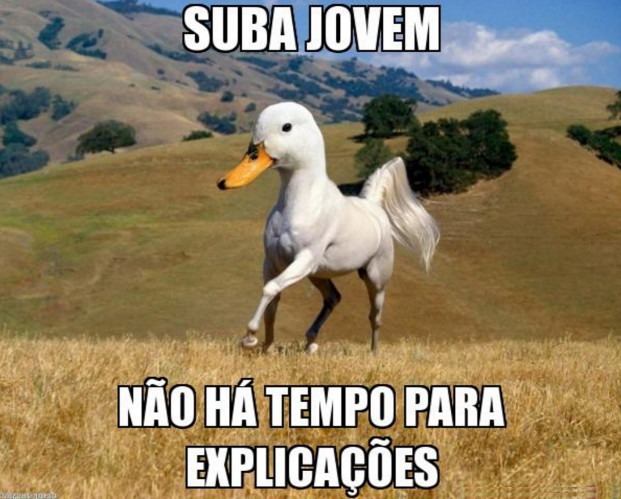
\includegraphics[width=50mm, right]{suba-jovem}
				\end{figure}
			\end{column}
			\begin{column}{0.55\textwidth}
				\vspace{7mm}
				\begin{itemize}
					\large
					\item[] Não entendeu o que é o Docker?
					\vspace{3mm}
					\item[] Tudo bem! Ficará mais claro quando a gente começar a usá-lo.
					\vspace{3mm}
					\item[] Por ora, apenas venham comigo!
				\end{itemize}
			\end{column}
			\begin{column}{0.05\textwidth}
			\end{column}
		\end{columns}
	\end{frame}

	\begin{frame}
		\frametitle{Instalação do Docker}
		Para matar a ansiedade, vamos dar um \textit{spoiler} da instalação do Docker:
		\begin{enumerate}
			\item Instalar o WSL (usuários Windows)
			\item Criar uma conta no \textit\textbf{DockerHub}
			\item Instalar o Docker Desktop
			\item Fazer o logon no app do Docker
			\item Baixar e executar uma imagem Docker 
		\end{enumerate}
	\end{frame}

	%Frame: Powershell installation [skipped]
	\begin{frame}<presentation:0>[noframenumbering]
		\frametitle{Microsoft PowerShell}
		\textbf{Passo 1:} Usuários do Windows também devem instalar o \textbf{Microsoft PowerShell}
		\vspace{0.6cm}
		\begin{columns}
			\column{0.07\textwidth}
			\column{0.15\textwidth}
			\begin{figure}[h]
				
\includegraphics[width=1.5cm]{powershell-icon.png}
			\end{figure}
			\column{0.80\textwidth}
			\begin{enumerate}
				\item Abra o prompt de comando e execute o winget para instalar o Microsoft PowerShell
				\lstinputlisting[style=winprompt]{winget-powershell.cmd}
				\vspace{0.4cm}
				\item Utilize a barra de pesquisas e procure pelo PowerShell. Verifique se o programa foi instalado corretamente.
			\end{enumerate}
			\column{0.60\textwidth}
		\end{columns}
	\end{frame}
	
	%Frame: Powershell screenshot [skipped]
	\begin{frame}<presentation:0>[noframenumbering]
		\frametitle{Microsoft PowerShell}
		\vspace{0.5cm}
		\begin{figure}[h]
			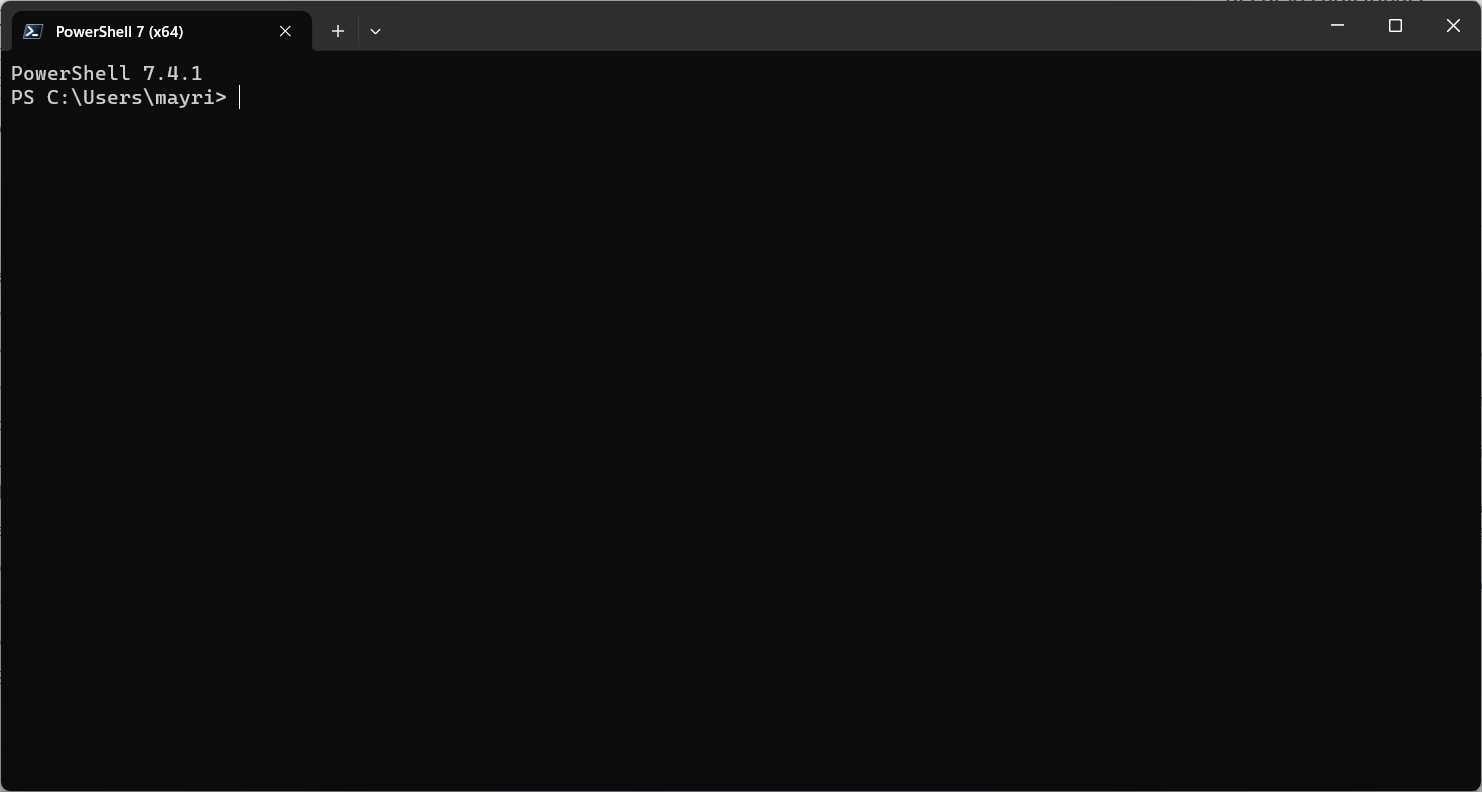
\includegraphics[width=0.70\textwidth]{powershell-window.png}
		\end{figure}
	\end{frame}

	%Frame: WSL2
	\begin{frame}
		\frametitle{Passo 1: instalar o WSL 2}
		\textbf{Pré-requisito:} antes de instalar o \textit{docker-desktop}, é necessário instalar o WSL (\textit{Windows Subsystem for Linux})
		\begin{enumerate}
			\item Abra o prompt de comando como administrador e execute o comando abaixo para instalar o wsl
			\lstinputlisting[style=winprompt]{wsl-install.cmd}
			\vspace{0.4cm}
			\item Depois terminar a execução do comando, você pode confirmar se a instalação foi bem sucedida, executando o comando wsl:
			\lstinputlisting[style=winprompt]{wsl-command.cmd}
		\end{enumerate}
	\end{frame}

	%Frame: Create Dockerhub account 
	\begin{frame}
		\frametitle{Passo 2: criar uma conta no DockerHub}
		Uma vez instalado o WSL, é hora de criar uma conta no DockerHub (caso ainda não tenha uma)
		\begin{enumerate}
			\item Vá até \href{https://hub.docker.com/signup}{\appallingunderline{https://hub.docker.com/signup}}
			\item Sigas instruções para criar uma conta (usuário, senha, email, etc..)
		\end{enumerate}
		\medskip
		\begin{figure}[h]
			\fbox{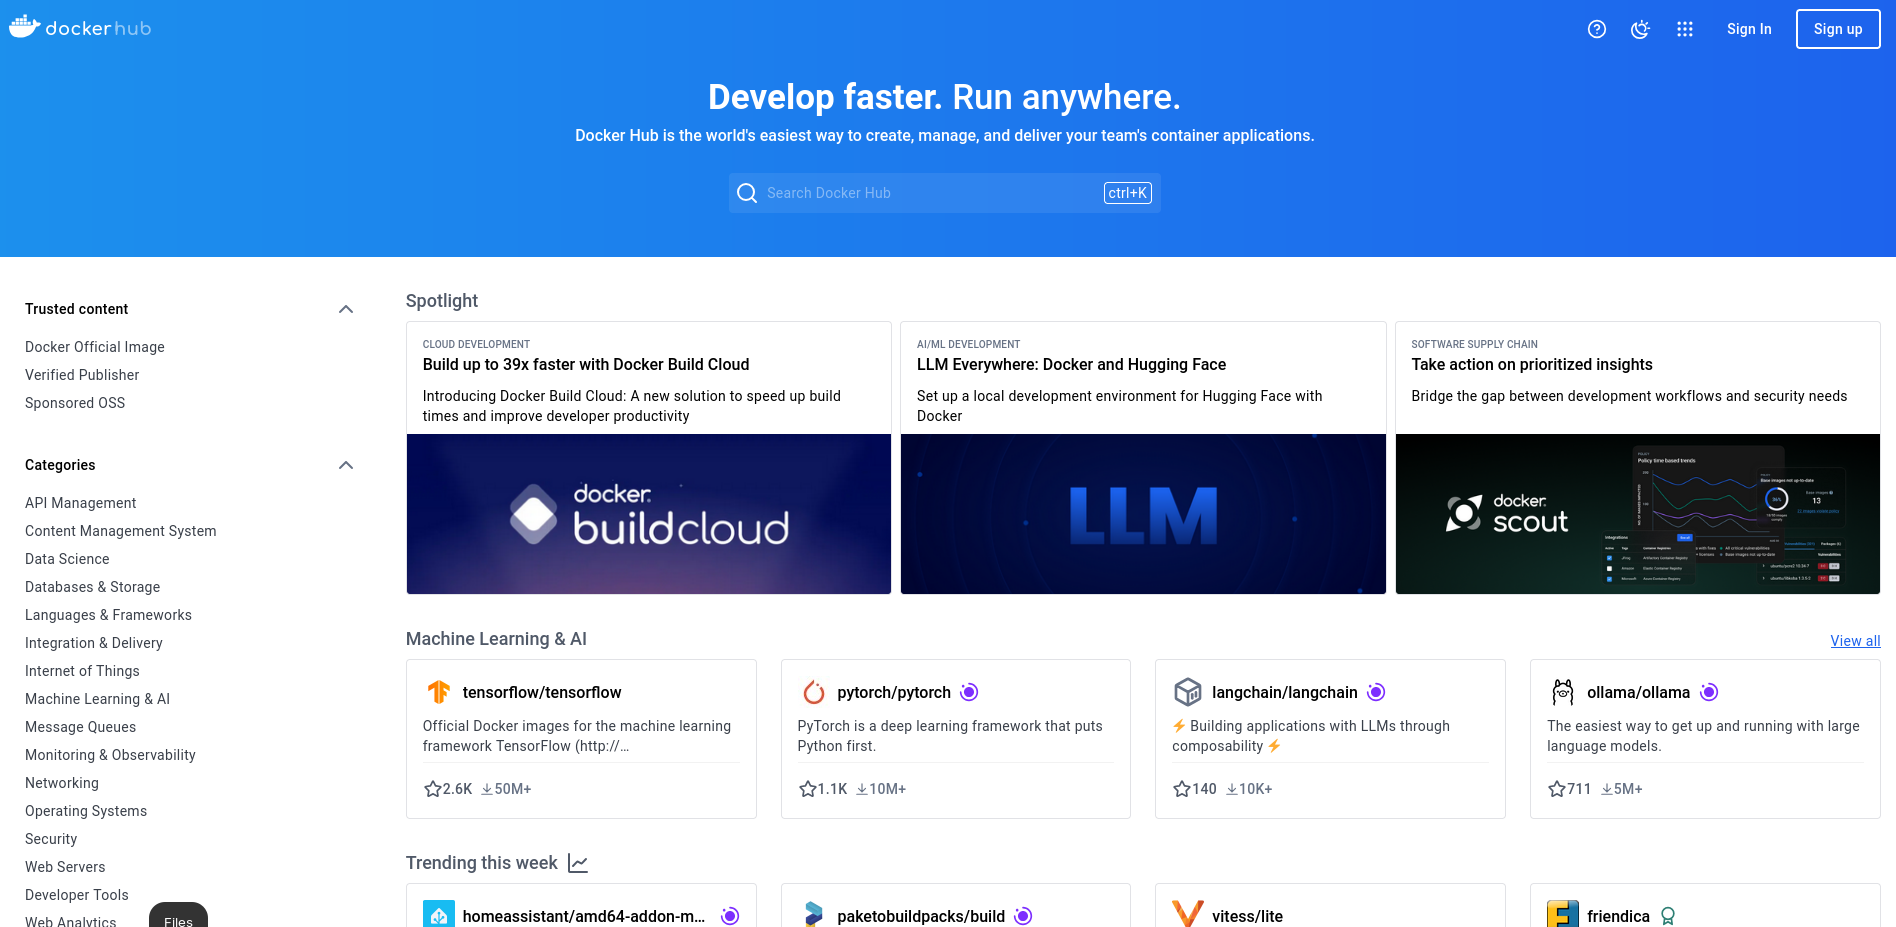
\includegraphics[height=42mm]{docker-hub-homepage.png}}
			\hspace{0.5cm}
			\fbox{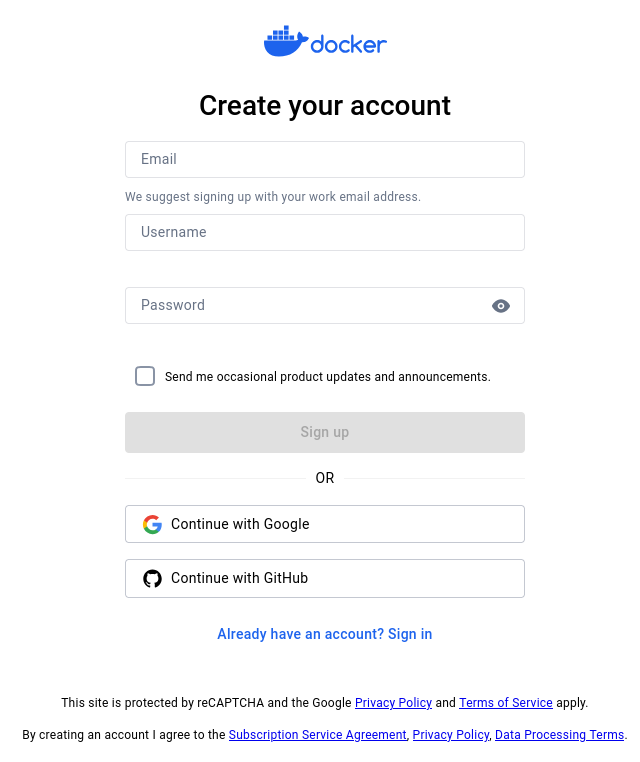
\includegraphics[height=42mm]{docker-signup.png}}
		\end{figure}
	\end{frame}

	%Frame: Docker Desktop Installation #1
	\begin{frame}
		\frametitle{Passo 3: Instalar do Docker Desktop}
		Uma vez instalado o WSL, podemos prosseguir para a instalação do Docker Desktop:
		\begin{enumerate}
			\item Vá até \href{https://www.docker.com/products/docker-desktop/}{\appallingunderline{https://www.docker.com/products/docker-desktop/}}
			\item Baixe o instalador do \textit{Docker Desktop} compatível com seu sistema
			\item Siga os passos de instalação
		\end{enumerate}
		\begin{figure}[h]
			\fbox{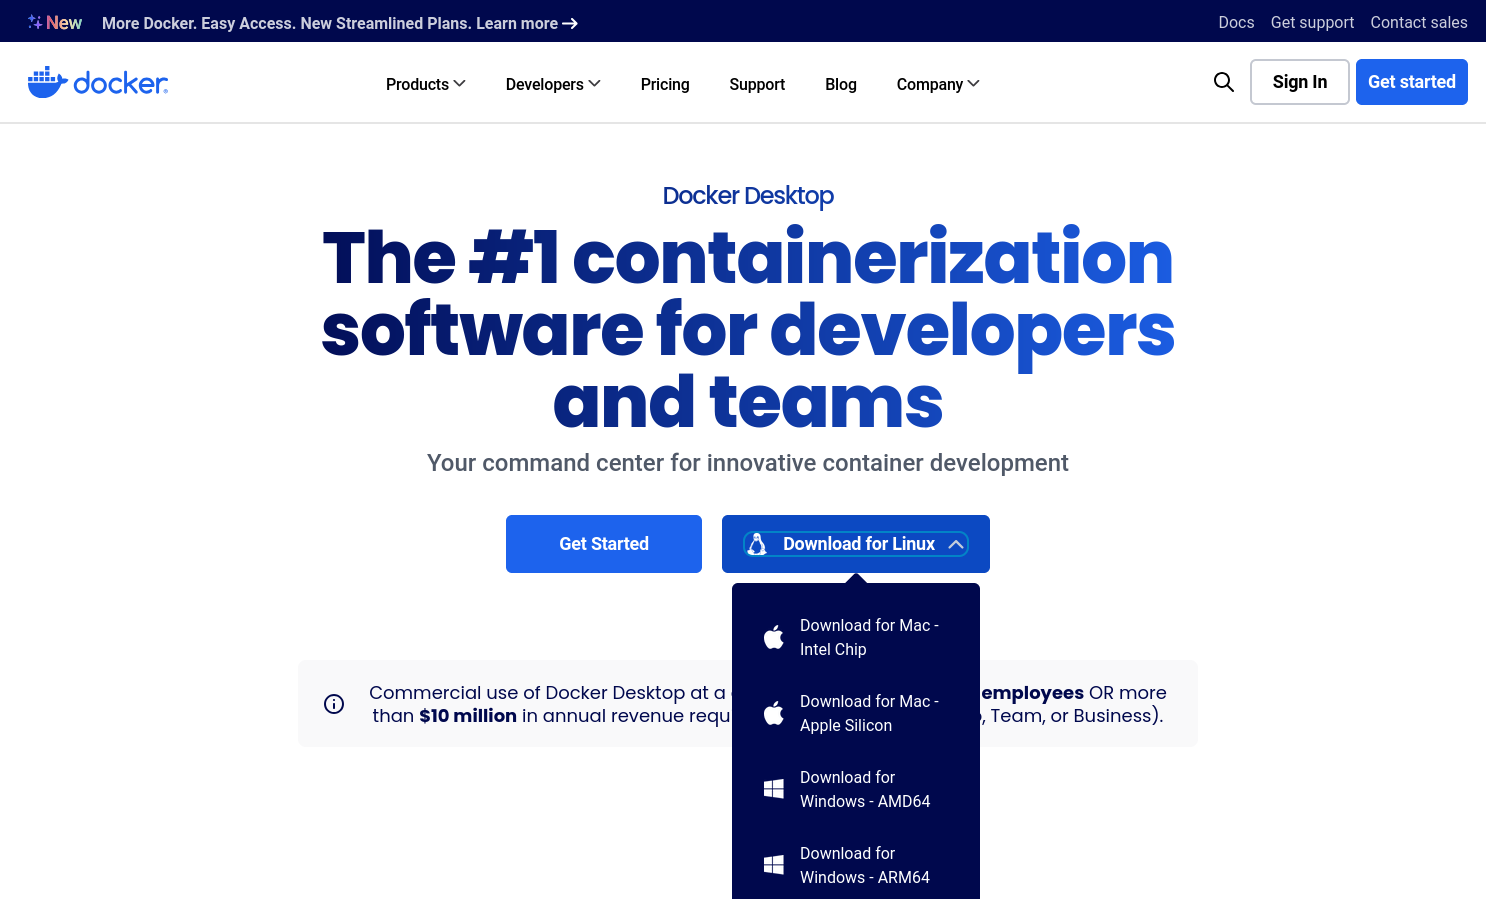
\includegraphics[height=38mm]{docker-desktop-download.png}}
			\hspace{0.5cm}
			\fbox{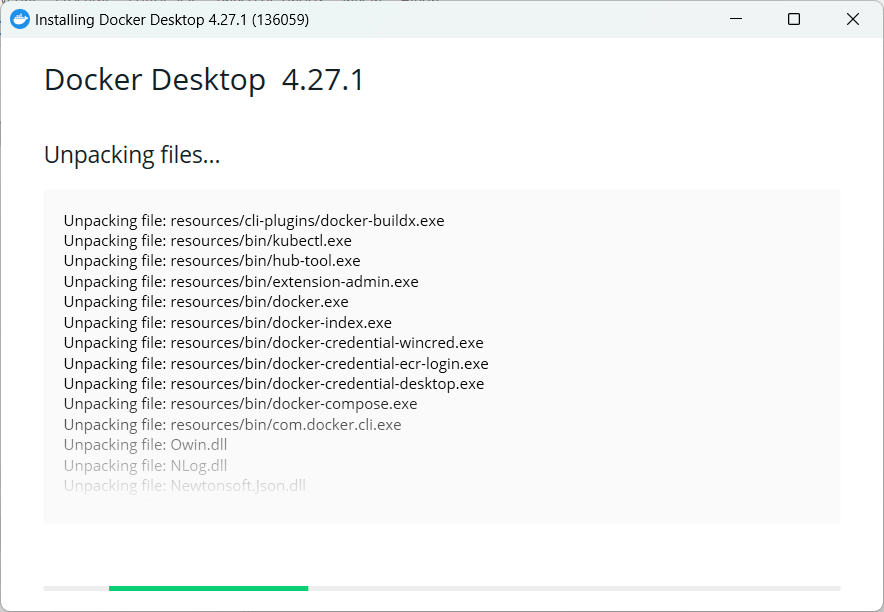
\includegraphics[height=38mm]{docker-installation.png}}
		\end{figure}
	\end{frame}
	
	%Frame: Docker Desktop Installation #1
	\begin{frame}
		\frametitle{Passo 3: Instalar do Docker Desktop}
		Depois de instalado, essa será a aparência do Docker:
		\begin{figure}[h]
			\fbox{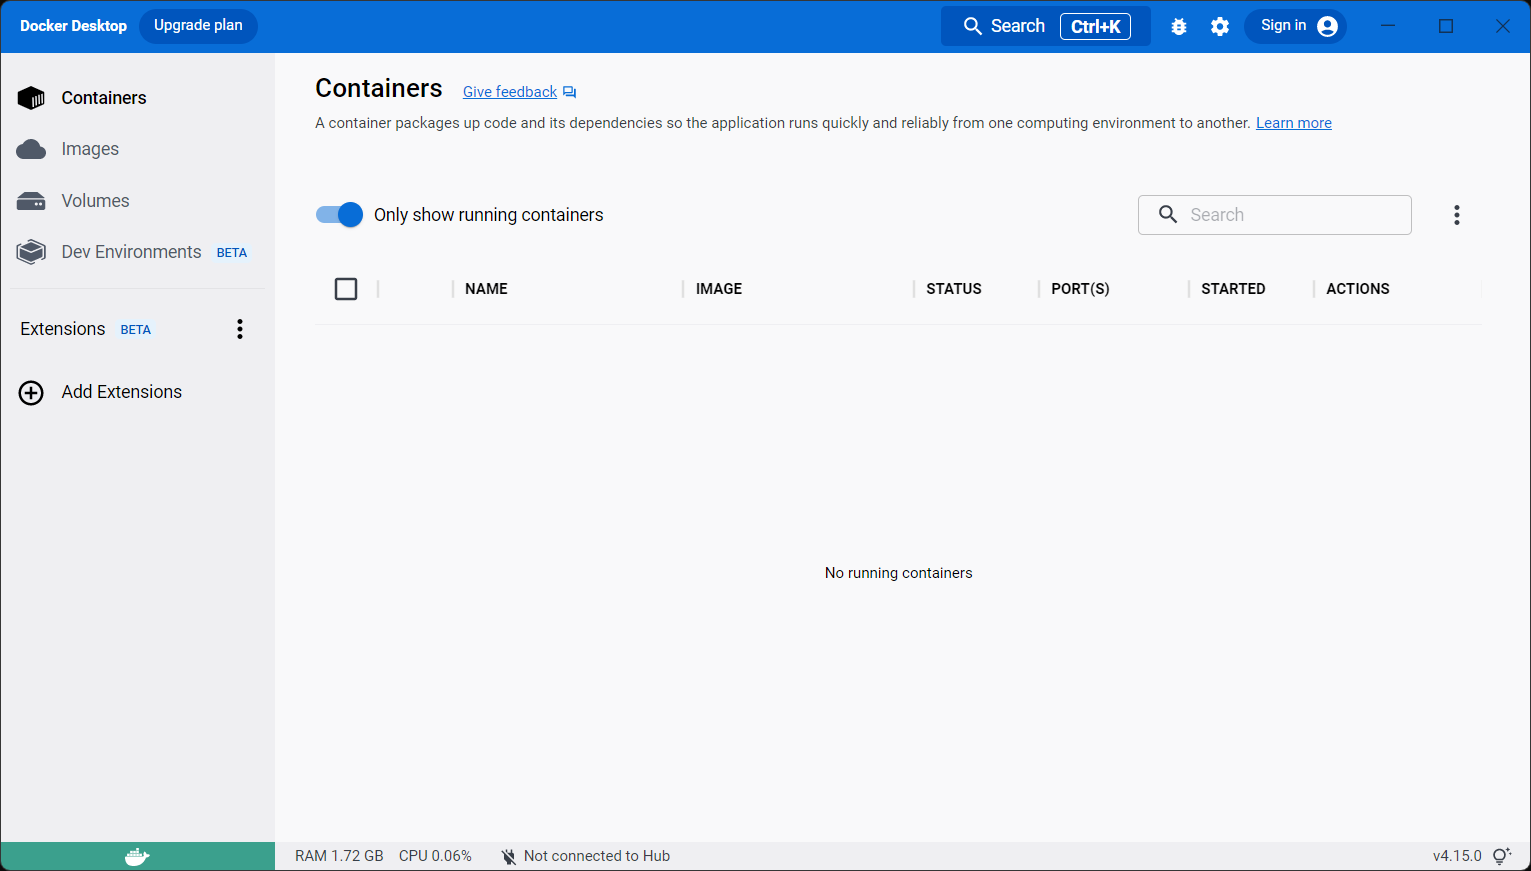
\includegraphics[width=0.70\textwidth]{docker-window.png}}
		\end{figure}
	\end{frame}

	%Frame: Docker Desktop Signin
	\begin{frame}
		\frametitle{Passo 4: Login no Docker Desktop}
		Dentro do Docker Desktop, você deve clicar em "Sign in" para se logar em sua conta do Docker Hub. 
		Você será redirecionad para fazer o login pelo navegador.
		\begin{figure}[h]
			\fbox{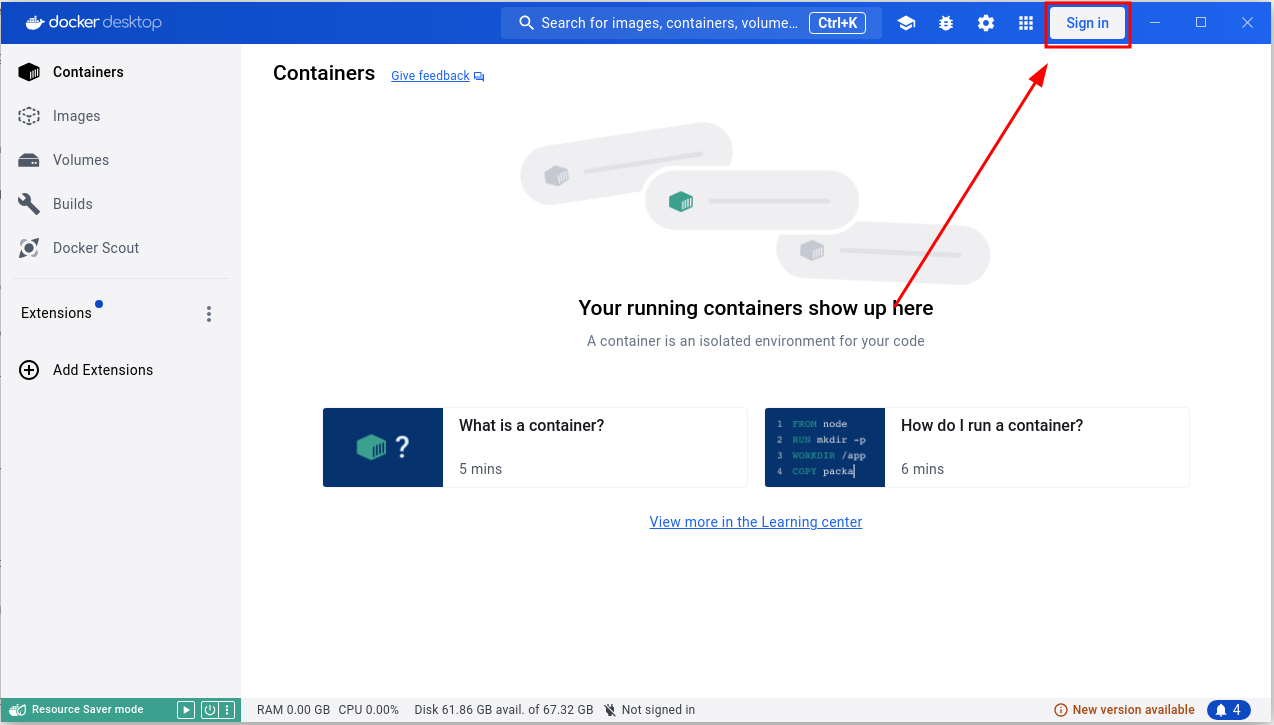
\includegraphics[width=0.70\textwidth]{docker-desktop-sign-in.png}}
		\end{figure}
	\end{frame}
	
	%Frame: Docker Desktop Signin
	\begin{frame}
		\frametitle{Passo 5: Baixar a imagem do MySQL}
		Vamos baixar a \textbf{imagem} do MySQL e executar um \textbf{container}
		\begin{itemize}
			\item \textbf{Imagem:} é a forma para fazer bolos
			\item \textbf{Container:} é um bolo feito a partir de uma forma
		\end{itemize}
		\begin{figure}[h]
			\fbox{
\includegraphics[height=45mm]{image-vs-container.png}}
		\end{figure}
	\end{frame}

	\section{Simulação do servidor MySQL}

	%Frame: emulating MySQL
	\begin{frame}
		\frametitle{Instalação das ferramentas}
		\vspace{0.5cm}
		\begin{center}
			\Large
			Muito bem, finalizamos a instalação das ferramentas! :D
		\end{center}
		\vspace{1cm}
		\begin{center}
			\LARGE
			Agora vamos iniciar a configuração! :(
		\end{center}
	\end{frame}
	
	\begin{frame}[t]
		\frametitle{Executando o MySQL com o database SakilaDB}
		Vamos utilizar o Docker para emular um banco de dados na nossa própria máquina.
		
		Clique na barra de pesquisa do Docker Desktop e procure pela imagem \textbf{\texttt{sakiladb/mysql}}
		\vspace{0.3cm}
		\begin{figure}[h]
			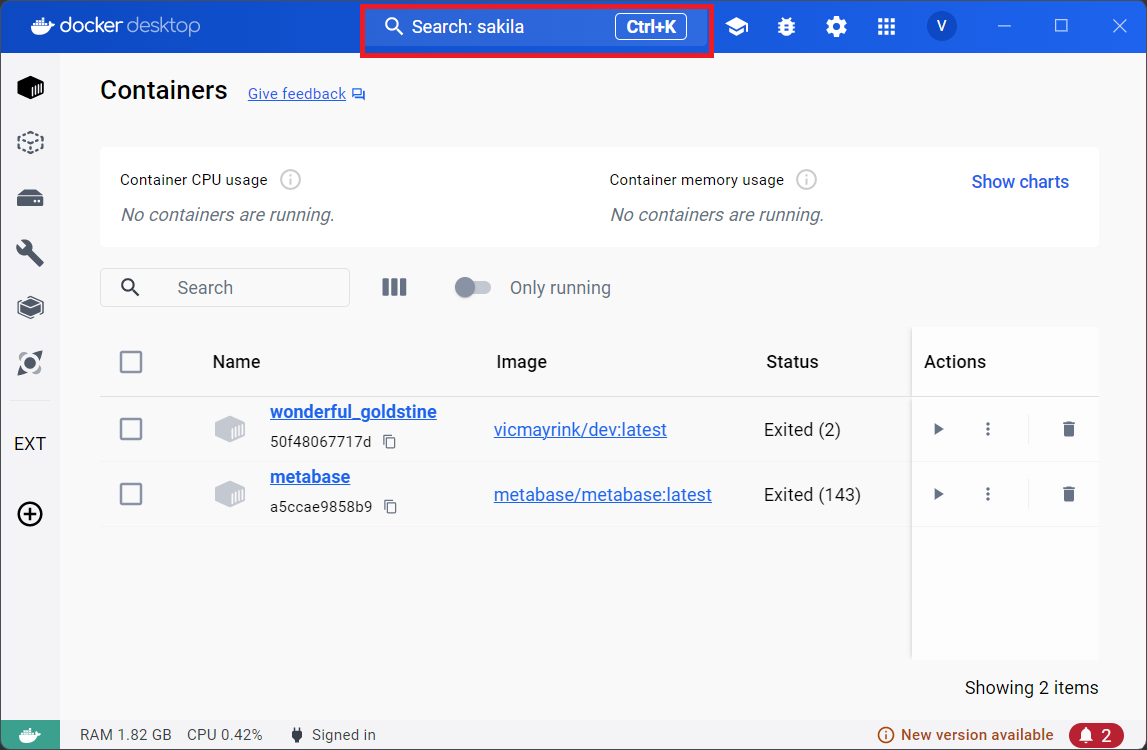
\includegraphics[width=0.45\textwidth]{docker-sakila-search-1.png}
			\hspace{0.5cm}
			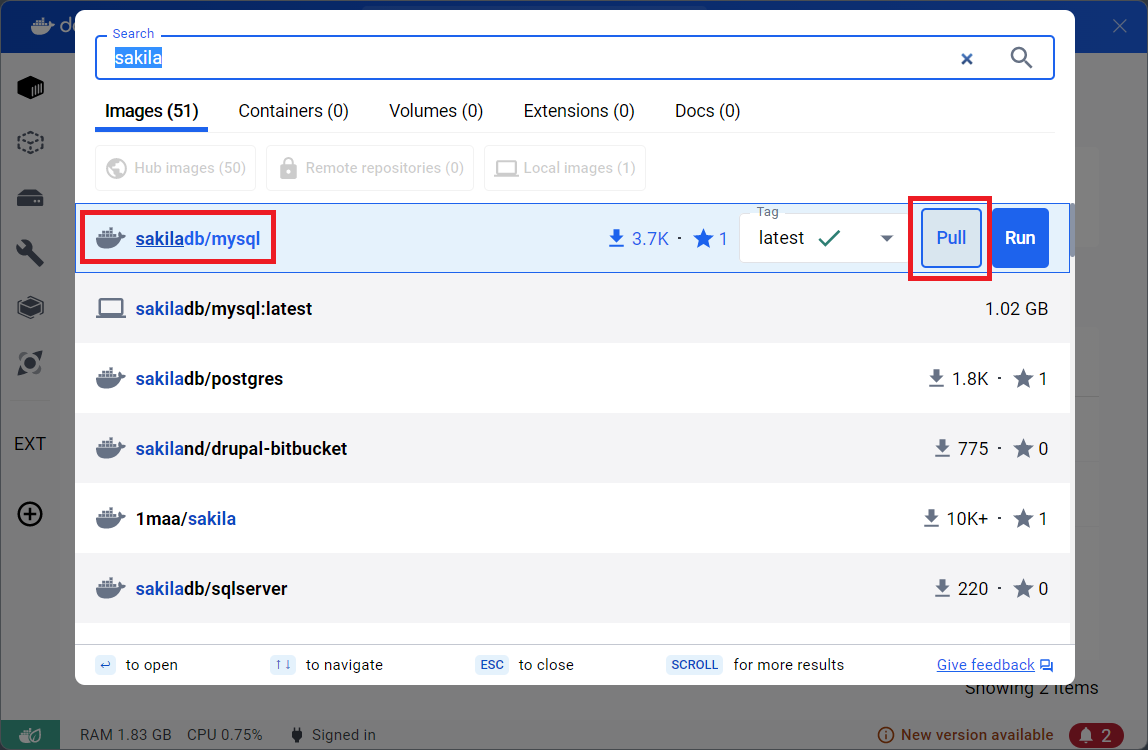
\includegraphics[width=0.45\textwidth]{docker-sakila-search-2.png}
		\end{figure}
	\end{frame}
	
	\begin{frame}[t]
		\frametitle{Executando o MySQL com o database SakilaDB}
		Ao executar o container do banco \textbf{\texttt{sakiladb}}, os logs são exibidos na tela.
		
		Os logs devem indicar quando o servidor \texttt{\textbf{MySQL}} estiver pronto para receber novas conexões.
		\vspace{0.1cm}
		\begin{figure}[h]
			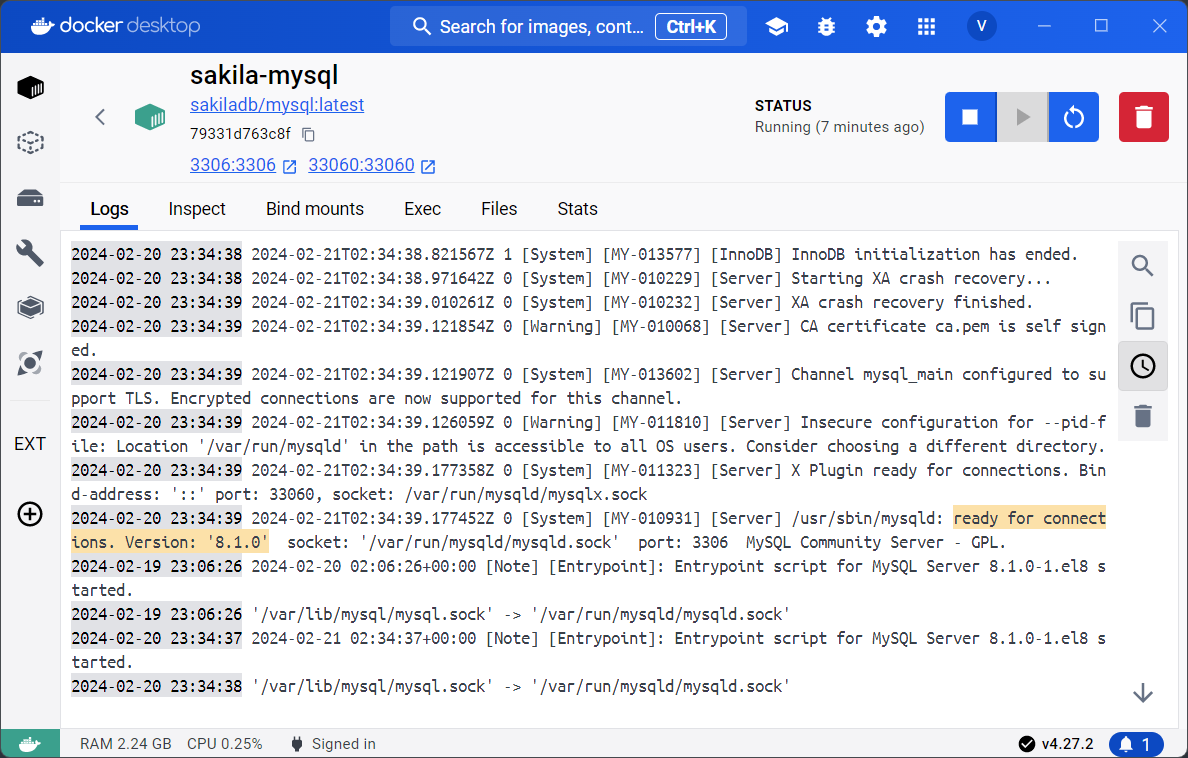
\includegraphics[width=0.55\textwidth]{docker-sakiladb-ready.png}
		\end{figure}
	\end{frame}

	\section{Conectando-se ao servidor MySQL}

	\begin{frame}[t]
		\frametitle{Conectando-se ao banco através do DBeaver}
		Agora vamos nos conectar ao banco de dados através do Dbeaver.
		
		\begin{enumerate}
			\small
			\item Abra o Dbeaver e clique em \texttt{Arquivo > Novo}
			\item Em seguida, selecione \texttt{Conexão com banco de dados}, dento do diretório Dbeaver
			\item Escolha o banco \texttt{\textbf{MySQL}} e clique em avançar
		\end{enumerate}
		
		\vspace{0.1cm}
		\begin{figure}[h]
			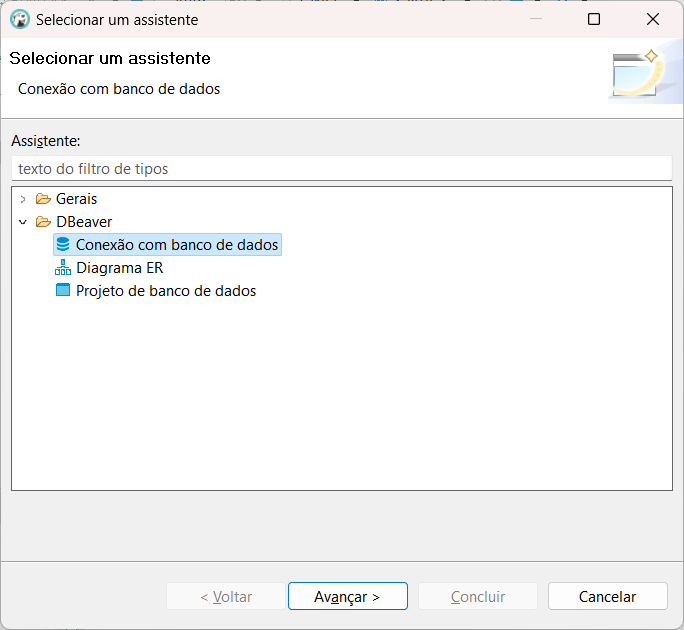
\includegraphics[width=0.32\textwidth]{dbeaver-new.png}
			\hspace{0.5cm}
			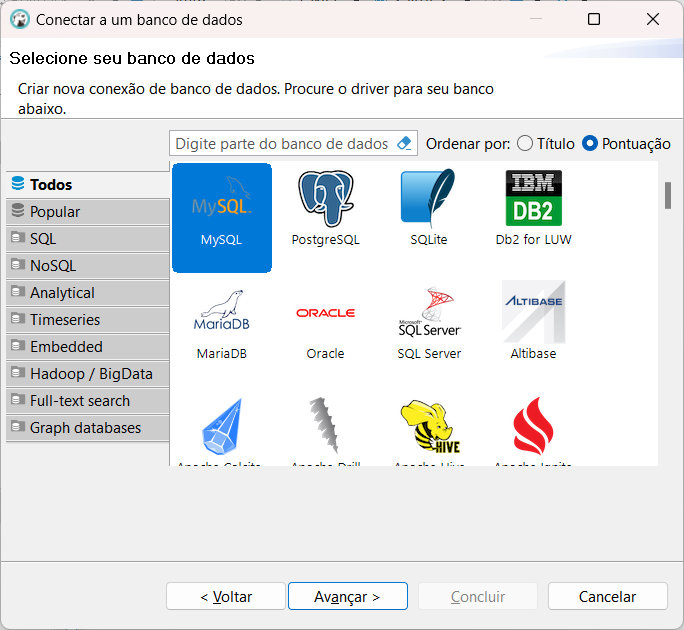
\includegraphics[width=0.32\textwidth]{dbeaver-db-select.png}
		\end{figure}
	\end{frame}
	
	\begin{frame}
		\frametitle{Conectando-se ao banco através do DBeaver}
		\vspace{0.05cm}
		\begin{columns}[t]
			\begin{column}{0.50\linewidth}
				\centering
				\begin{enumerate}
					\small
					\setcounter{enumi}{3}
					\item Preencha as credenciais de conexão, conforme a documentação da imagem do \textbf{\texttt{sakiladb}} que está em execução.
					\begin{itemize}
						\item \textbf{host:} localhost
						\item \textbf{port:} 3306
						\item \textbf{database:} sakila
						\item \textbf{user:} sakila
						\item \textbf{password:} p\_ssw0rd
					\end{itemize}
					\vspace{0.15cm}
					\item Finalmente clique em \texttt{Testar Conexão}
				\end{enumerate}
			\end{column}
			\begin{column}{0.45\linewidth}
				\begin{figure}[h]
					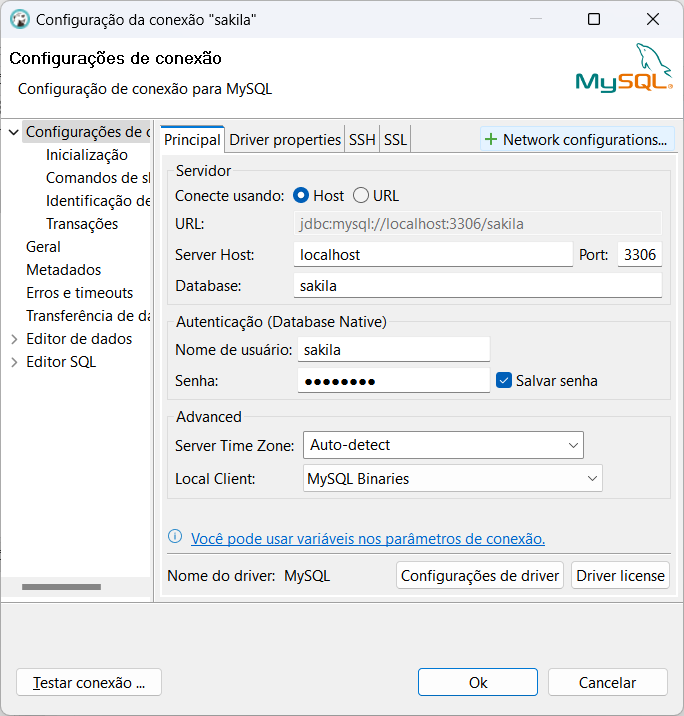
\includegraphics[width=0.85\textwidth, left]{dbeaver-edit-connection.png}
				\end{figure}
			\end{column}
		\end{columns}
	\end{frame}
	
\end{document}